\documentclass[11pt]{article}
\usepackage{fontspec}
\usepackage{amsmath,amssymb,amsthm,mathtools}
\usepackage[margin=1in]{geometry}
\usepackage{booktabs,array,tabularx}
\usepackage{enumitem}
\usepackage{xurl}
\usepackage{pgfplots}
\pgfplotsset{compat=1.18}
\usepackage[colorlinks=true,linkcolor=blue!50!black,citecolor=blue!50!black,urlcolor=blue!50!black]{hyperref}

\newtheorem{theorem}{Theorem}
\renewcommand{\thetheorem}{\Alph{theorem}}
\newtheorem{proposition}{Proposition}[section]
\newtheorem{lemma}[proposition]{Lemma}
\theoremstyle{remark}
\newtheorem{remark}[proposition]{Remark}

\newcommand{\Q}{\mathbb{Q}}
\newcommand{\F}{\mathbb{F}}
\newcommand{\lgn}{\lg n}
\DeclareMathOperator{\rank}{rank}
\DeclareMathOperator{\spn}{span}

\title{Integer multiplication below $n\log n$:\\ improving $\kappa$ from $2^{-182}$ to $2^{-59.335}$}
\author{Eray Yapağcı\thanks{The constructions, computations and text were produced by Claude Opus~5.5 (Anthropic) in an agentic Claude Code session directed by the author; see the repository README.}}
\date{October 7, 2026}

\begin{document}
\maketitle

\begin{abstract}
The OpenAI preprint \emph{Integer multiplication below $n\log n$} \cite{OAI} gives a deterministic multitape Turing machine that multiplies two $n$-bit integers in time $O(n(\lgn)^{1-\kappa})$ with $\kappa = 2^{-182}$; its constants are explicitly conservative. We keep the architecture of that algorithm and improve the exponent to $\kappa = 2^{-59.335}$ (any $\kappa < 2^{-58.329}$ is admissible before the paper's halving convention). Most of the gain comes from a new construction of the bit-level wire network that supplies the rank saving in the paper's chunk-interchange procedure: side wires become rectangles fed by copy wires whose label chains are shared across kernels, with cyclic point orders, giving $2h(h-3)^2$ copy chains per invocation. The remaining gain comes from re-tuned constants and three local changes to the cost accounting (axis exposure, the resampling parameter $\alpha$, and the guard depth). Every package is checked by an exact rational verifier, and the bit network is built gate-by-gate and checked for $h \le 16$. We also record structural limits (this architecture cannot pass about $\kappa \approx 2^{-50.5}$) and several negative results on alternative designs. This is computer-assisted work and has not been refereed.
\end{abstract}

\tableofcontents

\section{Introduction}\label{sec:intro}

Theorem~1 of \cite{OAI} gives one deterministic Turing machine, with a fixed finite alphabet and a fixed finite number of one-dimensional tapes, that multiplies two $n$-bit integers in time
\[
  T(n) = O\bigl(n(\lgn)^{1-\kappa}\bigr), \qquad \kappa = 2^{-182}.
\]
The constants in \cite[\S9.1]{OAI} are chosen ``deliberately conservative; no optimization is claimed''. This note asks how large $\kappa$ can be made while keeping the algorithm's architecture: the motif networks of \cite[\S3]{OAI}, the power-width interchange of \cite[Prop.~11]{OAI}, the simultaneous butterfly layers of \cite[Prop.~14]{OAI}, and the cost accounting of \cite[\S9]{OAI}.

\begin{theorem}[computer-assisted]\label{thm:main}
With the modifications of Sections~\ref{sec:outside} and~\ref{sec:bit}, the algorithm of \cite{OAI} runs in time $O(n(\lgn)^{1-\kappa})$ for every fixed $\kappa < 2^{-58.329}$. Following the convention of \cite[\S9.8]{OAI}, which takes $\kappa = \tfrac12\min_i g_i$ to leave explicit slack for fixed powers of $\log p$, this gives
\[
  \kappa = 2^{-59.335}.
\]
\end{theorem}

\paragraph{Status.} Theorem~\ref{thm:main} is supported by a proof outline (this note and the research notes in the repository \cite{repo}) together with exact machine verification of every numerical condition and gate-level checks of the new network for small parameters. It has not been refereed. The changes alter several procedures of \cite{OAI}, not only its constants. A complete proof would need a careful written argument for each change; Section~\ref{sec:status} lists precisely what is machine-checked and what is not.

\paragraph{Where the gain comes from.} Section~\ref{sec:accounting} shows that once the constants are re-tuned, $\kappa$ is determined almost entirely by one number: the saving exponent $\theta_b = 1-\tau$ of the \emph{bit} motif network, through $\kappa \approx \varepsilon\theta_b^2/2$ with $\varepsilon < 1/5$. The paper's bit network on $h = 100$ points has $\theta_b \approx 2^{-39.7}$; our final network has $\theta_b = 2^{-28.004}$. The improvement is staged as a sequence of packages, each adding to the previous one (Table~\ref{tab:packages}).

\begin{table}[ht]
\centering
\small
\begin{tabularx}{\textwidth}{@{}l l l l X@{}}
\toprule
Pkg & $\kappa$ & $\theta_b = 1-\tau$ & bit stages & change \\
\midrule
paper & $2^{-182}$ & --- & $h=100$ & published constants \\
A3 & $2^{-109.084}$ & $2^{-35.693}$ & 46 & re-tuned free constants (bit $h = 46$, complex $h = 25$) \\
B & $2^{-76.199}$ & $2^{-35.693}$ & 46 & axis exposure by $O(d)$ non-adjacent interchanges; guard $C_1 = 14$ \\
C & $2^{-74.978}$ & $2^{-35.693}$ & 46 & $\delta = 2^{-20}$; $\varepsilon < 1/4$; guard depth with leaf size $d^\beta$ \\
D & $2^{-73.733}$ & $2^{-35.071}$ & $(48,42,48)$ & per-stage designs; stage-1 scratch reused in stage 3 \\
E & $2^{-73.473}$ & $2^{-35.071}$ & $(48,42,48)$ & $\alpha = \lceil (8dp)^{1/4}\rceil$; $\varepsilon < 1/5$ \\
F & $2^{-70.142}$ & $2^{-33.407}$ & $(48,44,48)$ & grouped side-wire gates (sunflowers) \\
G & $2^{-68.616}$ & $2^{-32.644}$ & $(49,43,49)$ & laminar tree groups \\
H & $2^{-61.114}$ & $2^{-28.894}$ & $(51,48,51)$ & side rectangles fed by copy wires \\
I & $2^{-60.017}$ & $2^{-28.345}$ & $(51,50,51)$ & sorted-pattern rectangle cover \\
J & $2^{-59.591}$ & $2^{-28.130}$ & $(51,50,51)$ & copy chains shared across kernels \\
\textbf{K} & $\mathbf{2^{-59.335}}$ & $\mathbf{2^{-28.004}}$ & $(51,50,51)$ & cyclic per-kernel point orders \\
\bottomrule
\end{tabularx}
\caption{Verified packages. Every row is the exact output of \texttt{verification/scripts/verify.py}; each printed ``all constraints hold''.}
\label{tab:packages}
\end{table}

\begin{figure}[ht]
\centering
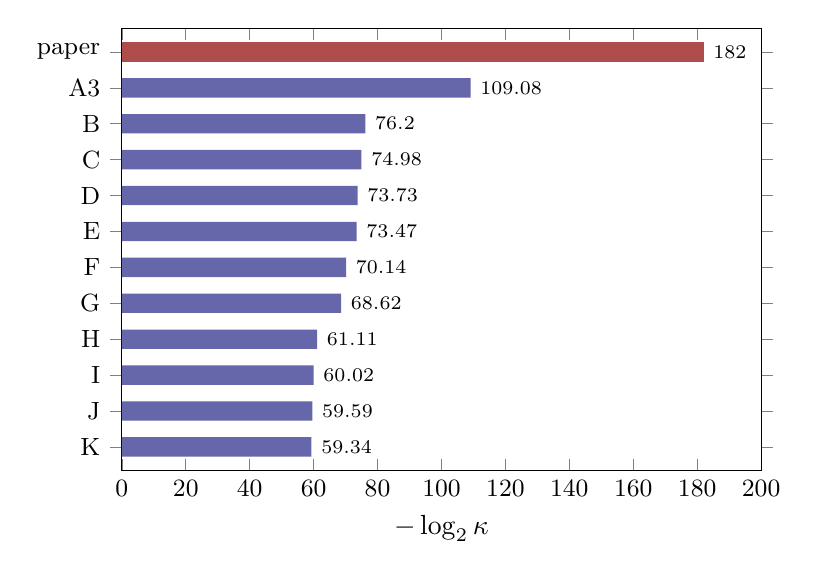
\begin{tikzpicture}
\begin{axis}[
  xbar, bar shift=0pt, width=0.8\textwidth, height=7.2cm,
  xmin=0, xmax=200,
  xlabel={$-\log_2 \kappa$},
  symbolic y coords={K,J,I,H,G,F,E,D,C,B,A3,paper},
  ytick={K,J,I,H,G,F,E,D,C,B,A3,paper}, y dir=normal,
  bar width=7pt,
  nodes near coords, nodes near coords align={horizontal},
  every node near coord/.append style={font=\scriptsize},
  enlarge y limits=0.06,
  tick label style={font=\small},
]
\addplot[fill=blue!45!black!60, draw=none] coordinates {
  (59.335,K) (59.591,J) (60.017,I) (61.114,H) (68.616,G) (70.142,F)
  (73.473,E) (73.733,D) (74.978,C) (76.199,B) (109.084,A3)
};
\addplot[fill=red!55!black!70, draw=none] coordinates {(182,paper)};
\end{axis}
\end{tikzpicture}

\caption{$-\log_2\kappa$ per package (shorter is better).}
\label{fig:bars}
\end{figure}

\paragraph{Lean.} No Lean formalization of \cite{OAI} exists in the OpenAI repository. The statement appears on the Lean FRO evaluation site \cite{LeanEval}. Nothing in this note is formalized.

\paragraph{Organization.} Section~\ref{sec:accounting} recalls the cost table and the rank condition and explains why $\theta_b$ binds. Section~\ref{sec:outside} describes the changes outside the bit network. Section~\ref{sec:bit} describes the new bit network. Section~\ref{sec:verification} describes the verification, Section~\ref{sec:limits} the structural limits and negative results, and Section~\ref{sec:status} the status of each claim.

\section{Where \texorpdfstring{$\kappa$}{kappa} comes from}\label{sec:accounting}

\subsection{The cost table and its margins}

Section~9.8 of \cite{OAI} divides every cost by $V = Tp = \Theta(n)$ and expresses it as a power of $p$, where $d = \Theta(p^\varepsilon)$ is the transform dimension, $\ell = \Theta(p^{1-\varepsilon})$ the axis width and $K = \Theta(p^{\varepsilon c})$ the chunk width \cite[(39)]{OAI}. Table~\ref{tab:costs} reproduces \cite[Table~1]{OAI} with our two modified rows. The margins below one are
\begin{equation}\label{eq:gaps}
\begin{gathered}
g_1 = 1-\varepsilon(1+c),\quad g_2 = \varepsilon c(1-\tau),\quad g_3 = \varepsilon(1-\lambda'),\quad g_4 = (1-\tau)(1-\varepsilon),\\
g_5 = \tfrac14 - \delta - \tfrac54\varepsilon,\quad g_6 = 1-\delta-\varepsilon,\quad g_7 = \varepsilon,
\end{gathered}
\end{equation}
which differ from \cite[(45)]{OAI} in $g_4$ (package B) and $g_5$ (package E). The time bound holds with any $\kappa < \min_i g_i$, because every fixed power of $\log p$ is absorbed by $p^{\min g_i - \kappa}$; \cite{OAI} takes $\kappa = \tfrac12 \min_i g_i$ and so do we.

\begin{table}[ht]
\centering
\small
\begin{tabular}{@{}lll@{}}
\toprule
Operation & normalized cost & power of $p$ \\
\midrule
Prefix-slot moves and individual butterfly rounds & $dK$ & $\varepsilon(1+c)$ \\
Chunk exchanges for transform layout & $pK^{\tau-1}$ & $1-\varepsilon c(1-\tau)$ \\
Simultaneous butterfly rounds & $\ell d^{\lambda'}$ & $1-\varepsilon(1-\lambda')$ \\
CRT and axis layouts (package B) & $d(1+\ell^\tau)$ & $\varepsilon + \tau(1-\varepsilon)$ \\
Gaussian line maps (package E) & $dp^{1/2+\delta}\alpha$ & $3/4+\delta+5\varepsilon/4$ \\
Chirps, twists and scalar products & $dp^\delta$ & $\varepsilon+\delta$ \\
Packed polynomial products & $\log(rp)$ & $1-\varepsilon$ \\
\bottomrule
\end{tabular}
\caption{\cite[Table~1]{OAI} with the rows changed by packages B and E. The paper's rows are $d^2(1+\ell^\tau)$ with power $\tau+\varepsilon(2-\tau)$, and $dp^{1/2+\delta}\alpha$ with power $3/4+\delta+3\varepsilon/2$.}
\label{tab:costs}
\end{table}

The parameters are also subject to the layer conditions of \cite[\S9.1]{OAI},
\begin{equation}\label{eq:layer}
\max\{\tau,\sigma\} < \lambda < 1,\qquad \tau(1+c/\beta) < \lambda,\qquad \max\{\lambda,\ \sigma+\beta(1-\sigma)\} < \lambda' < 1,
\end{equation}
and to the side conditions $c>0$, $0<\delta<1/8$, $\varepsilon(1+c)<1$, $\varepsilon+\delta<1$, together with the dimension and guard conditions discussed in Section~\ref{sec:outside}. Here $\tau$ and $\sigma$ are the interchange exponents supplied by the bit and complex motif networks.

\subsection{The rank condition}

A motif network is a circuit with $W$ wires and pointwise bit gates that realizes a permutation $\rho$ of its roles, together with rational $m\times m$ matrices on terminals and gates. With $A_e = M_{\mathrm{head}(e)} - M_{\mathrm{tail}(e)}$ for each edge $e$, the requirement \cite[(11)]{OAI} is
\[
M_{\mathrm{out}(\rho(w))} - M_{\mathrm{in}(w)} = I_m \quad (1\le w\le W), \qquad s = \sum_e \rank_\Q A_e < Wm,
\]
and \cite[Prop.~11]{OAI} then interchanges chunks in time $O(Ve^\tau)$ for every rational $\tau$ with $s/W < m^\tau$. Put
\[
\eta = 1 - \frac{s}{Wm}, \qquad \theta = 1-\tau .
\]
Any $\theta$ with $\theta\ln m < \eta$ is admissible, since then $m^{-\theta} > 1-\theta\ln m > 1-\eta = s/(Wm)$. The verifier picks a dyadic $\theta$ just below $\eta/\ln m$, with $\ln m$ bounded above by interval arithmetic.

For the label construction of \cite[\S3]{OAI}, every scratch wire is restored, each data pair saves exactly one rank at its endpoints, and decreasing edges occur only at centre wires. This gives
\begin{equation}\label{eq:s}
s = Wm - N + 2L, \qquad \eta = \frac{N-2L}{Wm},
\end{equation}
where $N$ is the number of data pairs and $L$ is the total dimension lost on decreasing edges \cite[Prop.~7]{OAI}. For the paper's bit network on $h=100$ points, $\theta_b \approx 2^{-39.74}$.

\subsection{Why the bit network binds}

The layer condition $\tau(1+c/\beta) < \lambda < 1$ forces $c < \beta\theta_b/(1-\theta_b)$, so $c \approx \theta_b$ and
\[
g_2 = \varepsilon c(1-\tau) \approx \varepsilon\theta_b^2 .
\]
Every other margin can be made much larger. The complex network enters only through $\sigma$ in \eqref{eq:layer}, and $g_3 = \varepsilon(1-\lambda') \approx \varepsilon(1-\beta)(1-\sigma)$ stays slack once $\beta$ is close to $1$. Margin $g_5$ caps $\varepsilon$ below $1/5$ (Section~\ref{sec:outside}). Hence
\[
\kappa \approx \tfrac12\varepsilon\theta_b^2 \approx \theta_b^2/10 .
\]
For package K, $\theta_b = 2^{-28.004}$ gives $\theta_b^2/10 \approx 2^{-59.33}$, which matches the verified value. Since $\kappa$ scales as $\theta_b^2$, each bit gained in $\theta_b$ is worth two bits of $\kappa$. Everything after package C is therefore about $\theta_b$.

The full parameter set of package K is
\begin{gather*}
1-\tau = 2^{-28.004},\quad 1-\sigma = 2^{-31.154},\quad c = 2^{-28.004}\ \text{(rounded)},\quad 1-\beta = 2^{-23.26},\\
\varepsilon = 0.199992,\quad \delta = 2^{-20} \approx 9.54\cdot 10^{-7},
\end{gather*}
with margins
\[
g_1 = g_6 = 2^{-0.322},\ g_2 = 2^{-58.329},\ g_3 = 2^{-56.735},\ g_4 = 2^{-28.326},\ g_5 = 2^{-16.830},\ g_7 = 2^{-2.322}.
\]
Then $\min g_i = g_2 = 2^{-58.329}$. Half of it, rounded down to a dyadic rational, is $\kappa = 2^{-59.335}$.

\section{Changes outside the bit network}\label{sec:outside}

\subsection{Package A3: re-tuned constants}
Package A3 leaves the algorithm unchanged. It reproduces the paper's network counts exactly (for $h=100$: $W_b$, $W_c$, $s_b$, $s_c$ as in \cite[\S3]{OAI}). It then chooses the ground-set sizes $h$ of the two motif networks and all fixed rationals in \eqref{eq:layer} and \cite[\S9.1]{OAI} to balance the margins: bit network $h=46$, complex network $h=25$. Under the paper's original conditions, in particular $\varepsilon(2-\tau) < 1-\tau$, this gives $\kappa = 2^{-109.084}$.

\subsection{Package B: axis exposure by non-adjacent interchanges}
In \cite[\S8]{OAI}, exposing and restoring one axis uses $O(d)$ \emph{adjacent} interchanges of address fields, each costing $O(Tp(1+\ell^\tau))$, so all axes cost $O(d^2)$ interchanges. This is the row $d^2(1+\ell^\tau)$ of the cost table, and it forces $\varepsilon(2-\tau) < 1-\tau$, i.e.\ $\varepsilon \lesssim \theta_b$.

Proposition~11 of \cite{OAI} interchanges two chunks of equal width with arbitrary fields between them, at the same cost as adjacent chunks. An axis can therefore be moved to the exposed position by a constant number of interchanges of non-adjacent chunks: peel one excess bit when the widths differ, as in \cite[\S8]{OAI}, and then interchange the equal-width parts directly. All $d$ axes then cost $O(d)$ interchanges. The row becomes $d(1+\ell^\tau)$ with power $\varepsilon + \tau(1-\varepsilon)$, so
\[
g_4 = (1-\tau)(1-\varepsilon),
\]
and $\varepsilon$ is no longer tied to $\theta_b$. Package B keeps the paper's guard $\varepsilon C_1 < 1$ of \cite[Prop.~14]{OAI} with $C_1 = \nu + 3 = 14$, where $\nu = 11$ is the least integer with $m_c^\nu \ge B_c = s_c + 64(W_c + m_c + 1)^3$ for the complex network. This gives $\varepsilon < 1/14$ and $\kappa = 2^{-76.199}$.

\subsection{Package C: $\delta$, the dimension bound and the guard depth}
\begin{itemize}[leftmargin=*]
\item Any fixed $0<\delta<1/8$ is allowed by Lemma~19 of \cite{OAI} and by \cite[Lemma~2.12]{HvdH}. We take $\delta = 2^{-20}$.
\item The convenience bound $\varepsilon < 1/12$ is replaced by what the proof uses: $\gamma = o(b)$ and $2 \le \alpha < \sqrt p$, which hold for $\varepsilon < 1/4$ with the paper's $\alpha$.
\item In the guard of \cite[Prop.~14]{OAI}, the leaves have size $e < d^\beta$, and there are at most $(1-\beta)\log_m d + 1$ internal levels and at most $md$ pieces. So the guard depth is $\Delta = d^{2+\beta+(1-\beta)\log_m B + o(1)}$, and the guard condition becomes
\[
\varepsilon\bigl(2+\beta+(1-\beta)\log_m B\bigr) < 1 .
\]
With $1-\beta = 2^{-23.26}$ this is far weaker than $\varepsilon C_1 < 1$. We keep the crude piece count $md$ from \cite{OAI}.
\end{itemize}
This gives $\kappa = 2^{-74.978}$.

\subsection{Package E: the resampling parameter $\alpha$}
Lemma~19 of \cite{OAI} needs $\theta_i = t_i/s_i - 1 > p/\alpha^4$ and $2 \le \alpha < \sqrt p$. Section~9.2.1 of \cite{OAI} sets $\alpha = \lceil (12 d^2 b)^{1/4}\rceil$ and uses $\theta_i > \eta = 1/(4d)$. We set instead
\[
\alpha = \bigl\lceil (8dp)^{1/4} \bigr\rceil .
\]
Then $\alpha^4\theta_i > 8dp/(4d) = 2p > p$, and $\gamma = 2d\alpha^2 = O(d^{3/2}p^{1/2}) = O(b^{1/2+3\varepsilon/2}) = o(b)$ for $\varepsilon < 1/3$. The Gaussian line maps then cost $dp^{1/2+\delta}\alpha = p^{3/4+\delta+5\varepsilon/4}$ instead of $p^{3/4+\delta+3\varepsilon/2}$, so $g_5 = 1/4 - \delta - 5\varepsilon/4$ and $\varepsilon$ may approach $1/5$. We take $\varepsilon = 1/5 - 2^{-17}$.

The constraint $\varepsilon < 1/5$ is in practice the end of the road for $\varepsilon$. The prime-interval requirement $\eta = 1/(4d)$ forces $\theta_i \approx 1/d$. Relaxing the Gaussian row all the way to the $\gamma$ bound $\varepsilon<1/3$ would add only about $0.74$ bits to $\kappa$.

\subsection{Package D: per-stage designs and scratch reuse}
Package D is described with the bit network in Section~\ref{sec:stages}.

\section{The bit network}\label{sec:bit}

\subsection{The paper's construction}\label{sec:paperbit}

We recall \cite[\S3]{OAI} in the form we need. Fix a ground set $[h]$, let $\mathcal T$ be its $v = \binom h3$ triples, and let $F = \Q^h$ carry the form $\langle x,y\rangle = x^{\mathsf T}(I-J/9)y$. With $t_T$ the indicator vector of $T$,
\[
\langle t_S, t_T\rangle = |S\cap T| - 1 ,
\]
so triple lines are nondegenerate and $t_S \perp t_T$ exactly when $|S\cap T| = 1$. The ambient label space is $F^{\otimes 3}$, of dimension $m = h^3$. Data roles are indexed by $a = (a_1,a_2,a_3)\in\mathcal T^3$, with $N = v^3$ data pairs $(X_a, Y_a)$.

The network has three stages. Stage $j$ acts along coordinate $j$ as $N/v$ independent \emph{invocations}, one for each value of the other two coordinates. An invocation is a network on the $v$ pairs $(x_T, y_T)_{T\in\mathcal T}$ that sends $y_T \mapsto y_T + x_T$ over $\F_2$ for every $T$, and restores all scratch wires whatever their initial values \cite[Lemma~5]{OAI}. It has two kinds of scratch wire.
\begin{itemize}[leftmargin=*]
\item \textbf{Centre wires.} For each point $q$, one wire gathers $\sum_{S\ni q}x_S$ and adds it to every $y_T$ with $T\ni q$. Together they add $C(S,T) = |S\cap T| \bmod 2$, which is $1$ on the diagonal and on pairs with $|S\cap T| = 1$, and $0$ otherwise. Each centre wire has one decreasing edge, which loses exactly $h$ dimensions.
\item \textbf{Side wires.} These cancel the off-diagonal ones of $C$. Each such \emph{cell} $(S,T)$ has $|S\cap T| = 1$, so it has a unique \emph{kernel} $q = S\cap T$, and $S = q+P$, $T = q+Q$ for disjoint pairs $P, Q$ of the other $n = h-1$ points. The paper uses one side wire per cell, i.e.\ $z = 3\binom{h-3}{2}$ per triple. Its label chain runs from $\langle t_S\rangle$ to $\langle t_T\rangle^\perp$ and is increasing because $t_S\perp t_T$.
\end{itemize}
With $I = 3v^2$ invocations, \cite[Prop.~7]{OAI} gives $W_b = 2N + I(vz + h)$ and $L_b = I\cdot h\cdot h$, and $s_b$ as in \eqref{eq:s}.

\subsection{Per-stage designs and scratch reuse (package D)}\label{sec:stages}

Nothing forces the three stages to use the same ground set. With stage $j$ on $h_j$ points ($v_j = \binom{h_j}3$), we get $m = h_1h_2h_3$, $N = v_1v_2v_3$, and stage $j$ has $N/v_j$ invocations. If $\mathrm{side}_j$ is the number of side and copy wires per invocation, then
\[
\mathrm{scr}_j = \frac{N}{v_j}\,(\mathrm{side}_j + h_j), \qquad L = \sum_{j=1}^3 \frac{N}{v_j}\,h_j^2 .
\]

\begin{lemma}[stage $1\to3$ reuse]\label{lem:reuse}
If $h_1 = h_3$, every stage-3 scratch wire can be a continuation of a stage-1 scratch wire with no loss. Hence $W = 2N + \mathrm{scr}_1 + \mathrm{scr}_2$.
\end{lemma}

\begin{proof}[Proof sketch]
A stage-1 scratch wire of invocation $(a_2,a_3)$ ends with label $F\otimes t_{a_2}\otimes t_{a_3}$. A stage-3 invocation $(a_1',a_2')$ has $\Pi = t_{a_1'}\otimes t_{a_2'}$ and $B = \Pi^\perp\subset F\otimes F$, and every one of its scratch wires starts at a label containing $B\otimes\langle t_{S'}\rangle$ (side wires) or equal to $B\otimes F$. If $|a_2\cap a_2'| = 1$, then $t_{a_2}\perp t_{a_2'}$, so $F\otimes t_{a_2}\subseteq B$. Hence the stage-1 end label lies inside the stage-3 start label (for side wires, choose $S' = a_3$). The continuation edge is increasing, and its residual is an orthogonal complement, hence nondegenerate. The bipartite graph joining $(a_2,a_3)$ to $(a_1',a_2')$ when $|a_2\cap a_2'| = 1$ is regular with equal supplies on both sides, so an integral $b$-matching assigns every stage-3 scratch wire to a distinct stage-1 wire.
\end{proof}

Continuing stage~1 into stage~2, or stage~2 into stage~3, is not free. The restore gates read $X$ after the centre gather, so scratch wires end at the full label, and continuing them costs one rank per wire.

\subsection{Grouped side gates (packages F and G)}

A gate may touch a data wire several times without creating new wires: in \cite{OAI} a wire is a source, the gates touching it in time order, and a sink. Packages F and G let one side wire serve a group of cells: sunflower groups of size at most $5$ (F), then laminar binary-tree groups per kernel (G). At $h = 48$, G reduces side wires to $0.181\,vz$. Package H supersedes both.

\subsection{Side rectangles and copy wires (package H)}

Fix an invocation and a kernel $q$. For a set $G$ of pairs of $[h]\setminus\{q\}$, write $q+G = \{q+P : P\in G\}$ and $\spn t_{q+G} = \spn\{t_{q+P}: P\in G\}$, and let $\operatorname{supp} G$ be the set of points covered by $G$.

\begin{lemma}[rectangle side wires]\label{lem:rect}
Let $G, H$ be sets of pairs with $\operatorname{supp} G\cap\operatorname{supp} H = \emptyset$. One wire that carries $\sum_{P\in G}x_{q+P}$ and adds it to every $y_{q+Q}$, $Q\in H$, has the increasing local label chain
\[
0 \ \subset\ \spn t_{q+G}\ \subseteq\ (\spn t_{q+H})^\perp\ \subset\ F
\]
and it cancels exactly the cells $(q+G)\times(q+H)$.
\end{lemma}

The middle inclusion holds because every $S\in q+G$, $T\in q+H$ meet only in $q$, so $t_S\perp t_T$. Over $\F_2$ the side wires must cancel each cell an odd number of times; we use partitions. The sums $\sum_{P\in G}x_{q+P}$ are formed on \emph{copy wires} and the results are scattered through \emph{accumulators}. A copy wire passes through a sequence of nodes, and its label must increase along the way, so the nodes on one copy wire must form a chain under span inclusion. The number of copy wires that triple $S$ needs on the source side is therefore the Dilworth width \cite{Dilworth} of the set of source nodes containing $S$, and similarly on the target side. The data wires $X_S$ and $Y_S$ themselves serve as one chain each. Per invocation,
\begin{equation}\label{eq:side}
\mathrm{side} = \#\text{rectangles} + \#\text{source chains} + \#\text{target chains} - 2\binom h3 .
\end{equation}
Every node label must be nondegenerate for $I-J/9$; this is checked explicitly (Section~\ref{sec:verification}).

\subsection{The sorted cover (package I)}

Order the $n$ points of $[h]\setminus\{q\}$. For a cell with $P = (x_1<x_2)$ and $Q = (z_1<z_2)$, the rectangle is chosen by the interleaving pattern, using the node families
\begin{align*}
\mathrm{Wpre}(z) &= \{(a,b) : b<z\}, & \mathrm{rowfrom}(x) &= \{(x,b)\},\\
\mathrm{rowsuf}(x,z) &= \{(x,b): b>z\}, & \mathrm{colpre}(z,x) &= \{(a,x): a<z\},\\
\mathrm{colmid}(z,x) &= \{(a,x): a>z\}.
\end{align*}

\begin{center}
\small
\begin{tabular}{@{}lll@{}}
\toprule
pattern & source node $G$ & target node $H$ \\
\midrule
$x_2<z_1$ (PPQQ) & $\mathrm{Wpre}(z_1)$ & $\mathrm{rowfrom}(z_1)$ \\
$z_2<x_1$ (QQPP) & $\mathrm{rowfrom}(x_1)$ & $\mathrm{Wpre}(x_1)$ \\
$x_1<z_1<x_2<z_2$ (PQPQ) & $\mathrm{colpre}(z_1,x_2)$ & $\mathrm{rowsuf}(z_1,x_2)$ \\
$z_1<x_1<z_2<x_2$ (QPQP) & $\mathrm{rowsuf}(x_1,z_2)$ & $\mathrm{colpre}(x_1,z_2)$ \\
$x_1<z_1<z_2<x_2$ (PQQP) & $\mathrm{rowsuf}(x_1,z_2)$ & $\mathrm{colmid}(x_1,z_2)$ \\
$z_1<x_1<x_2<z_2$ (QPPQ) & $\mathrm{colmid}(z_1,x_2)$ & $\mathrm{rowsuf}(z_1,x_2)$ \\
\bottomrule
\end{tabular}
\end{center}

Each rule's $G$ and $H$ have disjoint supports, and each cell lies in exactly one rectangle $G\times H$ (both facts are asserted by the code). The cover uses about $3.76\binom n2$ rectangles per kernel: $4606$ at $n = 50$ and $4416$ at $n = 49$. The per-kernel chain width is $3$. At $n = 47$ it uses $4048$ rectangles against an $\F_2$-rank lower bound of $3960$ for the four interleaved order types, so it is within $2.2\%$ of that bound.

\subsection{Chains across kernels (packages J and K)}

A copy wire needs only nested spans along its route, and equal spans are allowed. A triple $S = \{q,a,b\}$ has nodes in the three kernels $q,a,b$. A node in kernel $q$ that consists of all triples through $\{q,a\}$ spans the same space as a node in kernel $a$ with the same triple set. So one copy wire may pass through nodes of different kernels of $S$, provided all nodes are visited in one global time order. We order nodes globally by (span rank, key) and compute, for each triple, the Dilworth width of all its source (target) nodes over its three kernels.

\paragraph{Package J (one global point order).} The interior width drops from $3+3+3 = 9$ to $7$ per side. The total number of source chains per invocation is
\[
\tfrac16\bigl(7h^3 - 39h^2 + 26h + 102\bigr),
\]
fitted on $h = 14,\dots,20$ and exact for $h = 9,\dots,13, 15, 26, 30, 34$.

\paragraph{Package K (cyclic point orders).} Kernel $q$ orders the other points as $q+1, q+2, \dots, q-1 \pmod h$. Let the cyclic gaps of a triple be $(g_1,g_2,g_3)$, with $g_1+g_2+g_3 = h$. The width per side is
\[
\begin{cases}
6 & \text{if all } g_i\ge 2,\\
3 & \text{if exactly one } g_i = 1 \text{ (2 for one composition per position)},\\
2 & \text{if two } g_i = 1 .
\end{cases}
\]
Summing over triples gives
\[
\tfrac h3\Bigl[6\tbinom{h-4}{2} + 3\bigl(3(h-5)+2\bigr) + 6\Bigr] = h(h-3)^2
\]
per side. This is exact for $h = 9,\dots,19, 23, 26, 31$. Hence, by \eqref{eq:side},
\[
\mathrm{side}_K(h) = h\cdot\mathrm{rects}(h-1) + 2h(h-3)^2 - 2\binom h3 .
\]
Simulated annealing over independent per-kernel orders and a hill climb over cyclic offsets did not find a better order (Section~\ref{sec:limits}).

\subsection{Stages 2 and 3}

Stage~2 is the dual network: its gates run in reverse order (the $\F_2$ gates are involutions), the $X$ and $Y$ banks swap roles, and every local label $U$ becomes $U^\perp$. Inclusions and time both reverse, so chains stay nested and the centre loss is unchanged. Stage $j\ge 2$ embeds local labels by $U\mapsto B\otimes F + \Pi\otimes U$ (in stage~1, $B = 0$ and $\Pi$ is trivial), which is monotone and preserves nondegeneracy. Every scratch wire still starts at $B\otimes F$ and ends at $A\otimes F$ (with $A\supset B$ the ambient space of the other two factors), so Lemma~\ref{lem:reuse} still applies.

\subsection{Final counts}

For package K with stages $(51,50,51)$, the cover has $\mathrm{rects}(50) = 4606$ and $\mathrm{rects}(49) = 4416$, so
\[
\mathrm{side}_K(51) = 428264 \ (= 20.565\,v_1), \qquad \mathrm{side}_K(50) = 402500 \ (= 20.536\,v_2),
\]
and
\begin{gather*}
N = 8\,500\,140\,250\,000,\qquad m = 130\,050,\qquad W = 366\,403\,749\,643\,750,\\
L = 3\,207\,501\,902\,500,\qquad s = 47\,650\,805\,556\,033\,242\,500,
\end{gather*}
giving $2L < N$, $s < Wm$, $\eta = 4.3759\cdot 10^{-8}$ and $\theta_b = 2^{-28.004}$.

\section{Verification}\label{sec:verification}

All code is in \texttt{verification/} of the repository \cite{repo}.

\paragraph{The constraint verifier (\texttt{scripts/verify.py}).} For each package it recomputes $W$, $L$, $s$, $\eta$ and $\theta$ for both motif networks as exact rationals. It then evaluates every condition of Sections~\ref{sec:accounting} and~\ref{sec:outside} with exact fractions, using rigorous interval bounds (\texttt{mpmath.iv}) only for $\ln m$ and $\log_m B$. It prints the margins $g_1,\dots,g_7$. Before any change it reproduces the paper's $h = 100$ counts exactly (\texttt{scripts/networks.py}). The run is deterministic: \texttt{make verify} regenerates \texttt{data/verify\_all.txt} byte for byte.

\paragraph{Gate-level network checks (\texttt{scripts/check\_copy.py}, \texttt{scripts/check\_cross.py}).} These build one complete invocation of the bit network: every wire, gate and label, with labels as explicit subspaces of $\Q^h$ computed modulo the prime $p = 1\,000\,003$. They check that:
\begin{enumerate}[leftmargin=*]
\item over $\F_2$, for random inputs and random initial scratch values, the network maps $y\mapsto y+x$ and restores $x$ and every scratch wire;
\item along every wire the label sequence (source, gates in time order, sink) is nested, and the only decreasing edges are the centre edges, each losing $h$;
\item every gate label is nondegenerate for $I - J/9$;
\item the wire counts equal the formulas of Section~\ref{sec:bit}.
\end{enumerate}
With \texttt{DUAL=1} they build the stage-2 dual network instead.

\begin{center}
\small
\begin{tabular}{@{}lll@{}}
\toprule
construction & stage 1 & stage 2 (dual) \\
\midrule
sorted cover, per-kernel chains (I) & $h = 8, 10, 11, 12, 13, 14$ & $h = 8, 10, 12, 13$ \\
global cross-kernel chains (J) & $h = 8, 10, 12$ & $h = 8, 10, 12$ \\
cyclic cross-kernel chains (K) & $h = 8, 10, 12, 14, 16$ & $h = 8, 10, 12, 14, 16$ \\
\bottomrule
\end{tabular}
\end{center}

For package K the copy counts equal $2h(h-3)^2 - 2\binom h3$ exactly ($288, 740, 1504, 2660, 4288$). At $h = 16$ the check covers $10\,800$ nested wires and $6\,402$ distinct nondegenerate labels. The value $h = 9$ is excluded because $I - J/9$ is itself degenerate there; this is irrelevant at $h\in\{50,51\}$. As a negative control, a deliberately invalid support rule (\texttt{scripts/bad\_supp.py}) fails the checker.

\paragraph{Formula confirmation.} The final value at $h \in\{50,51\}$ uses the counting formulas, not an explicit network. Rectangle counts $\mathrm{rects}(n)$ are computed exactly by enumerating the cover (\texttt{data/sorted\_*.txt}, for $30\le n\le 56$). The chain formulas were confirmed by exact Dilworth-width computation up to $h = 31$ (K) and $h = 34$ (J).

\section{Structural limits and negative results}\label{sec:limits}

\subsection{Limits of this architecture}
\begin{itemize}[leftmargin=*]
\item \textbf{Three stages are forced.} The endpoint identity needs the swap $\rho(X_a) = Y_a$, which takes three shears, each exposing one tensor factor. Hence $m = h_1h_2h_3$.
\item \textbf{$\kappa\approx\varepsilon\theta_b^2/2$ is structural.} A breakpoint argument (each swap fixes at most four boundaries, and runs start at width $K$) shows that contiguous-block layouts need about $Dq/8$ swaps of width at least $K$. So the layout cost $pK^{\tau-1}$ cannot be improved by such swaps, and $g_2 = \varepsilon c(1-\tau)$ with $c\approx\theta_b$ remains.
\item \textbf{The centre is near-optimal.} Every centre wire loses exactly $h$ whatever it gathers, so the centre loss is $c\cdot h$ per invocation. Here $c$ is the minimum $\F_2$-rank of a matrix with unit diagonal that vanishes on pairs with $|S\cap T|\in\{0,2\}$. Restricting to a pencil gives $c\ge h-2$. A CP-SAT search shows $c = 6$ is infeasible at $h = 8$, so at most about $1/h$ of $L$ could be saved. Block centres collapse to singletons under the parity of $4$-sets, and order-type centre rules force the paper's star centre.
\item \textbf{Headroom.} With stages $(51,50,51)$ re-optimized at each point, side wires per triple of $26.2$, $13.1$, $7$, $3$ and $0$ give $\kappa = 2^{-60.00}$, $2^{-58.11}$, $2^{-56.47}$, $2^{-54.47}$ and $2^{-50.48}$. Package K sits at $20.6$. So even free side wires would not take this architecture past about $2^{-50.5}$.
\end{itemize}

\subsection{Negative results}
\begin{itemize}[leftmargin=*]
\item \textbf{$\F_q$ labels.} The triple graph ($|S\cap T| = 1$) contains a Kneser graph $K(n-1,2)$. A topological bound \cite{Haviv} gives orthogonality dimension at least $n-3$ over every field, so there is no gain.
\item \textbf{Rectangle merging.} Merging rectangles that share a source or target set saves only about $2\%$ at $h = 10, 12$, because union nodes break chains elsewhere. Merging all twin rectangles at $h = 10$ removes $150$ rectangles but adds $590$ chains.
\item \textbf{Other point orders.} Reverse, alternating, zig-zag and mid-rotation orders are all worse. Simulated annealing over independent per-kernel orders (about $47\,000$ evaluations at $h = 8, 10$) and an 80-minute cyclic-offset hill climb at each of $h = 10, 12$ all ended at the cyclic order.
\item \textbf{Rule variants.} Variants of the cover rules, per-kernel mixing of variants, and type-separated keys give identical or worse totals.
\item \textbf{Endpoint and cycle savings.} A rank bound allows endpoint savings of up to $\dim V$ per data pair, or about $m$ per $\rho$-cycle of scratch roles. No realizable routing was found.
\end{itemize}

\subsection{Different per-coordinate designs}
To escape the ceiling of about $2^{-50.5}$ we also changed the per-coordinate design itself. In a generic design, $v$ elements carry labels of dimension $f$ (or $k$-dimensional label subspaces, with $\xi = f/k$), the centre has $\F_2$-rank $c$, and each element carries $w$ scratch wires. Then
\[
\eta \approx \frac{1-6/R}{\xi^3(2+2w)}, \qquad R = \frac{v}{c\,\xi};
\]
for triples, $\xi = h$ and $R = h/6$.
\begin{itemize}[leftmargin=*]
\item \textbf{$7$-subsets with a degree-$3$ centre} ($C = \binom{|S\cap T|}{3}\bmod 2$, side pairs $|S\cap T| = 3$). The ceiling is higher, but each element has $35$ kernels, each a disjointness instance on $4$-sets. Each kernel needs at least $5$ copy chains per side (a hyperplane-covering bound), so an element needs at least about $175$ scratch wires against a budget of about $200$--$300$. No cover approaching this was found.
\item \textbf{Other polynomial and product designs.} The design $(s,d,e) = (15,7,1)$ has worse side covers. Product designs give $R = \xi/36$. $\F_3$ labels do not help.
\item \textbf{Subspace (vector-linear) labels.} If each triple received a $k$-dimensional subspace with $\xi\approx h/2$, $\eta$ would grow about $18$-fold at $h = 51$. A numerical search (L-BFGS over all real signatures) at $h = 10$, $k = 2$ finds $f = 14$ and $16$ infeasible, does not reach $f = 18$, and confirms $f = 20 = 2h$. A complex scalar representation lifts to a rational one with $k = 2$, and the real $k=2$ runs at $h = 8$ match the complex ones exactly, so we computed the complex symmetric minrank of the triple graph directly. It equals $h$ for $h = 7$ and $h = 10, 11, 12$ (rank $h-1$ fails), and rank $11$ also fails at $h = 13$. It equals $h-1$ at $h = 8$ and $h = 9$. The $h = 8$ solution is the Steiner system $S(3,4,8)$: seven orthogonal classes of eight triples. Colourings of this kind cost about $h^2/6$ dimensions for large $h$. These lower bounds are numerical evidence, not proofs.
\end{itemize}

\section{Status of the claims}\label{sec:status}

\begin{itemize}[leftmargin=*]
\item \textbf{Machine-checked exactly.} All numerical conditions for every package (exact rationals with interval logarithms). The bit-network constructions of packages I, J and K, built gate by gate for the parameters listed in Section~\ref{sec:verification}: $\F_2$ correctness, nested label chains, nondegenerate labels and wire counts. Rectangle counts for $30\le n\le 56$, which include the values $n = 49, 50$ used here.
\item \textbf{Confirmed by computation but not proved.} The closed forms for the chain counts (J up to $h = 34$, K up to $h = 31$), which are then used at $h = 50, 51$. A proof of $h(h-3)^2$ from the cyclic-gap classification of Section~\ref{sec:bit} would close this gap; we have the classification but not a written proof of the widths.
\item \textbf{Argued in outline only.} The changes to the procedures of \cite{OAI}: non-adjacent axis exposure (B), the guard depth with leaf size $d^\beta$ (C), the choice of $\alpha$ (E), stage-$1\to3$ scratch reuse (D), and the transfer of the new network into \cite[Prop.~11]{OAI}. The research notes in the repository contain the arguments as they were developed. Each needs a careful written proof before the result should be relied on.
\item \textbf{Not independent.} The verifier is our own transcription of the constraint system of \cite{OAI}. It reproduces the paper's network counts exactly, but it is not independent of our reading of the paper.
\end{itemize}

Nothing here is formalized in Lean.

\paragraph{How this was produced.} The constructions, searches and verification code were produced by Claude Opus~5.5 (Anthropic), working as an agent in an extended Claude Code session, directed by the author. Errors in the outline arguments are possible, and corrections are welcome.


\bibliographystyle{plain}
\bibliography{references}
\end{document}
